\documentclass[]{article}
\usepackage{amssymb,amsmath}
\usepackage{ifxetex,ifluatex}
\ifxetex
  \usepackage{fontspec,xltxtra,xunicode}
  \defaultfontfeatures{Mapping=tex-text,Scale=MatchLowercase}
\else
  \ifluatex
    \usepackage{fontspec}
    \defaultfontfeatures{Mapping=tex-text,Scale=MatchLowercase}
  \else
    \usepackage[utf8]{inputenc}
  \fi
\fi
\usepackage{url}
\usepackage{graphicx}
% We will generate all images so they have a width \maxwidth. This means
% that they will get their normal width if they fit onto the page, but
% are scaled down if they would overflow the margins.
\makeatletter
\def\maxwidth{\ifdim\Gin@nat@width>\linewidth\linewidth
\else\Gin@nat@width\fi}
\makeatother
\let\Oldincludegraphics\includegraphics
\renewcommand{\includegraphics}[1]{\Oldincludegraphics[width=\maxwidth]{#1}}
\ifxetex
  \usepackage[setpagesize=false, % page size defined by xetex
              unicode=false, % unicode breaks when used with xetex
              xetex,
              colorlinks=true,
              linkcolor=blue]{hyperref}
\else
  \usepackage[unicode=true,
              colorlinks=true,
              linkcolor=blue]{hyperref}
\fi
\hypersetup{breaklinks=true, pdfborder={0 0 0}}
\setlength{\parindent}{0pt}
\setlength{\parskip}{6pt plus 2pt minus 1pt}
\setlength{\emergencystretch}{3em}  % prevent overfull lines
\setcounter{secnumdepth}{0}

\author{Bob Benjamin}

\begin{document}

\newcommand{\truncateit}

{[}1{]}\truncate{0.8\textwidth}{#1}

\newcommand{\scititle}

{[}1{]}

\newcommand{\vdag}{(v)^\dagger}

\newcommand{\av}{$A_{V}$}

\newcommand{\mav}{A_{V}}

\newcommand{\degrees} {$^\circ$}

\newcommand{\kms}{km\ s$^{-1}$}

\newcommand{\cc}{cm$^{-3}$}

\newcommand{\cmsq}{cm$^{-2}$}

\newcommand{\htwo}{${\rm H_2}$}

\newcommand{\mhtwo}{{\rm H_2} }

\newcommand{\cotwoone}{$^{12}$CO~(2-1)}

\newcommand{\co}{$^{12}$CO}

\newcommand{\ammonia}{${\rm NH}_3$}

\newcommand{\thco}{$^{13}$CO}

\newcommand{\mco}{ {\rm ^{12}CO}}

\newcommand{\mthco} { {\rm ^{13}CO}}

\newcommand{\wthco}{$W(\mthco)$}

\newcommand{\nthco}{$N(\mthco)$}

\textbf{Abstract}. The very long, thin infared dark cloud ``Nessie" is
even longer than had been previously claimed, and an analysis of its
Galactic location suggests that it lies directly in the Milky Way's
mid-plane, tracing out a highly elongated bone-like feature within the
prominent Scutum-Centaurus spiral arm. Re-analysis of mid-infrared
imagery from the Spitzer Space Telescope shows that this IRDC is at
least 2, and possibly as many as 8 times longer than had originally been
claimed by Nessie's discoverers, \citet{Jackson2010}; its aspect ratio
is therefore at least 150:1, and possibly as large as 800:1. A careful
accounting for both the Sun's offset from the Galactic plane ($\sim 25$
pc) and the Galactic center's offset from the $(l^{II},b^{II})=(0,0)$
position defined by the IAU in 1959 shows that the latitude of the true
Galactic mid-plane at the 3.1 kpc distance to the Scutum-Centaurus Arm
is not $b=0$, but instead closer to $b=-0.5$, which is the latitude of
Nessie to within a few pc. Apparently, Nessie lies \emph{in} the
Galactic mid-plane. An analysis of the radial velocities of low-density
(CO) and high-density (${\rm NH}_3$) gas associated with the Nessie dust
feature suggests that Nessie runs along the Scutum-Centaurus Arm in
position-position-velocity space, which means it likely forms a dense
`spine' of the arm in real space as well. No galaxy-scale simulation to
date has the spatial resolution to predict a Nessie-like feature, but
extant simulations do suggest that highly elongated over-dense filaments
should be associated with a galaxy's spiral arms. Nessie is situated in
the closest major spiral arm to the Sun toward the inner Galaxy, and
appears almost perpendicular to our line of sight, making it the easiest
feature of its kind to detect from our location (a shadow of an Arm's
bone, illuminated by the Galaxy beyond). Although the Sun's offset from
the Galactic plane is not significant compared with the thickness of the
plane as traced by Population I objects such as GMCs and HII regions, it
may be significant compared with an extremely thin layer that might be
traced out by Nessie-like objects. Future high-resolution extinction and
molecular line data may therefore allow us to exploit the Sun's position
above the plane to gain a small amount of perspective on the Galactic
disk.

\textbf{Instructions for Co-Authors} \emph{(will be deleted later--other
readers please skip this section)}

\begin{itemize}
\item
  Still-needed text/contributions/thoughts from specific co-authors are
  marked with ``xx."
\item
  The full file repository for this paper is at
  \url{https://drive.google.com/#folders/0BxIRxiTe1u6BcGlnUGt2ckU1Vms},
  shared with all co-authors.
\item
  The ``aas" (press conference) slides at
  \url{https://drive.google.com/#folders/0BxIRxiTe1u6BRklQRzlUaUNuUUU}.
\item
  The Mendeley Library "NessieandFriends" used to house references used
  in this work, at:
  \url{http://www.mendeley.com/groups/2505711/nessie-and-friends/}.
\item
  The Glue software used to intercompare data sets used in this work is
  online through: \url{http://glueviz.org}.
\item
  We are using \url{http://Authorea.com} as an experimental platform to
  compile this paper.
\item
  There are also some oddities in the Mendeley-generated .bib file (and
  alphabetization), so we will need to clean up the referencing and
  bibliography by hand when we submit this paper.
\end{itemize}
\section{Introduction}

Determining the structure of the Milky Way, from our vantage point
within, is a perpetual challenge for astronomers. We know the Galaxy has
spiral arms, but it remains unclear exactly how many, cf.
\citep{Vallee2008a}. Recent observations of maser proper motions give
unprecedented accuracy in determining the three-dimensional position of
the Galaxy's center and rotation speed \citep{Reid2009,Brunthaler2011}.
But, to date, we still do not have a definitive picture of the Milky
Way's three dimensional structure.

The analysis offered in this paper suggests that some infrared dark
clouds (The term ``Infrared Dark Cloud" or ``IRDC" typically refers to
any cloud which is opaque in the mid-infrared.) --in particular very
long, very dark, clouds--appear to delineate the major features of our
Galaxy as would be seen from outside of it. In particular, we study a
$>3^{\circ}$-long cloud associated with the IRDC called ``Nessie"
\citep{Jackson2010} and we show that it appears to lie parallel to, and
no more than just few pc from, the true Galactic Plane.

Our analysis uses diverse data sets, but it hinges on combining those
data sets with a modern understanding of the meaning of Galactic
coordinates. When, in 1959, the IAU established the current system of
Galactic $(l,b)$ coordinates \citep{Blaauw1959}, the positions of the
Sun with respect to the ``true" Galactic disk, and of the Galactic
Center, were not as well determined as they are now. As a result, the
Galactic Plane is typically \textbf{not} at $b=0$, as projected onto the
sky. The exact offset from $b=0$ depends on distance, as we explain in
§{[}lookingdown{]}. Taking these offsets into account, one can
profitably re-examine data relevant to the Milky Way's 3D structure. The
Sun's vantage point slightly ``above" the plane of the Milky Way offers
useful perspective.

IRDCs are loosely defined as clouds with column densities high enough to
be obvious as patches of significant extinction against the diffuse
galactic background mid--infrared wavelengths. This implies that IRDCs
are relatively starless: if they were to contain bright IR sources and
nebulosity, they would not stand out as dark clouds. To give examples,
\citet{Peretto2009a} draw the boundaries of IRDCs at an optical depth of
0.35 at $8~\rm{}\mu{}m$ wavelength, equivalent to an $\rm{}H_2$ column
density $\approx{}10^{22}~\rm{}cm^{-2}$. In their sample, clouds have
average column densities of a few $10^{22}~\rm{}cm^{-2}$ (e.g., Figure~2
of \citealt{peretto2010:irdcs-mass-density}). Some IRDCs do actively
form high--mass stars (e.g., \citealt{pillai2006:g11} and
\citealt{rathborne2007:irdc-msf}). It is therefore thought that some
IRDCs are future sites of high--mass star formation.
\citet{kauffmann2010:irdcs} demonstrate that most IRDCs are not massive
and dense enough to form high--mass stars \citep{kauffmann2010:irdcs}.
Still, they also argue that the few $10^2$ most massive and dense clouds
may contain a large fraction of the star--forming gas in the Milky Way.
In that case, a small number of very dense and massive IRDCs may be
responsible for a large fraction of the galactic star formation rate.
The massive stars forming in these dense IRDCs are so bright, that
extragalactic observers of the Milky Way might see IRDCs hosting young
massive stars as the predominant mode of star formation here. Thus, if
one can deduce the pattern of IRDCs that an observer outside the Milky
Way would see, one can determine the Milky Way's (non-dark-matter)
structure, from inside. (CB Note: these last 2 sentences are interesting
-- does it contradict Jens' claims made about star forming efficiencies
in IRDCs? Jens: changed text to highlight that high--mass SF is limited
to the most massive and dense IRDCs. Then the argument still holds that
bright stars may trace IRDCs. If this is to hold for Nessie, this cloud
should exceed the mass--size limit from \citep{kauffmann2010:irdcs}.)

The traditional ISM-based probes of the Milky Way's structure have been
HI and CO. Emission in these tracers gives line intensity as a function
of velocity, so the position-position-velocity data resulting from HI
and CO observations can give three dimensional views of the Galaxy, if a
rotation curve is used to translate line-of-sight velocity into a
distance. Unfortunately, though, the Galaxy is filled with HI and CO, so
it is very hard to disentangle features when they overlap in velocity
along the line of sight. Nonetheless, much of the basic understanding of
the Milky Way's spiral structure we have now comes from HI and CO
observations of the Galaxy, much of it from the compilation of CO data
presented by \citet{Dame2001}.

Recently, several groups have targeted high-mass star-forming regions in
the plane of the Milky Way for high-resolution ISM observations. In
their BeSSeL Survey, Reid et al. are using hundreds of hours of VLBA
time to observe hundreds of regions for maser emission, which can give
both distance and kinematic information for very high-density ($n>10^8$
cm$^{-3}$) gas \citep{Reid2009,Brunthaler2011}. In the HOPS Survey,
hundreds of positions associated with the dense peaks of infrared dark
clouds have now been surveyed for ${\rm NH}_3$ emission
\citep{Purcell2012b}, yielding high-spectral resolution velocity
measurements towards gas whose density typically exceeds $10^4$
cm$^{-3}$. In follow-up spectral-line surveys to the ATLASGAL dust-based
survey of the Galactic Plane \citep{Beuther2012a}, \citet{Wienen2012}
have measured ${\rm NH}_3$ emission in nearly 1000 locations. The
ThrUMMs Survey aims to map the entire fourth quadrant of the Milky Way
in CO and higher-density tracers \citep{BarnesPeter2010}, which also
holds the potential for more high-resolution velocity measurements.

Targets in the high-resolution velocity studies are usually identified
based on continuum surveys, which show the locations of the highest
column-density regions, either as extinction features (``dark clouds" in
the optical, ``IRDCs" in the infrared), as dust emission features (in
surveys of the thermal infrared), or as gas emission features (e.g. HII
regions).

Great power lies in the careful combination of continuum and
spectral-line data when one wants to understand the structure of the ISM
in three-dimensions. Thus, there have already been several efforts to
combine dust maps with spectral-line data, whose goal is often the
assignment of more accurate distances to particular clouds or regions
e.g., \citep{Foster2012}. These improved distances allow for more
reliable conversion of measured quantities (e.g. fluxes) to physical
ones (e.g. mass).

In this study, our aim is to combine morphological information from
large-scale mid-infrared continuum ``dust" maps of the Galactic Plane
with spectral-line data, so as to understand the nature of very long
infrared dark clouds that appear parallel to the Galactic Plane. We
focus in particular on the IRDC named ``Nessie" in the study presented
by \citet{Jackson2010}. In that 2010 paper, Nessie is shown to be a
highly elongated filamentary cloud (see Figure {[}fig:FindingChart{]})
exhibiting the after-effects of a sausage instability that led to
several massive-star-forming peaks spaced at regular intervals. We
extend the work of Jackson et al. by first by literally ``extending" the
cloud, to a length of at least 3 degrees (§{[}longer{]}). In §{[}3D{]},
we show that a careful accounting for the modern measures of the Sun's
height off of the Galactic mid-plane and of the true position of the
Galactic Center imply that Nessie lies not just parallel to the Galactic
Plane, but \emph{in} the Galactic Plane. We consider what
velocity-resolved measures of the material associated with Nessie tells
us about its three-dimensional position in the Galaxy, and we conclude,
in §{[}spine{]} that Nessie likely marks the ``spine" of the
Scutum-Centaurus arm of the Milky Way in which it lies. In
§{[}future{]}, we consider, in the light of coming computational and
observational capabilities, the likelihood of finding more
``Nessie-like" structures in the future, and of using them, in
conjunction with the Sun's vantage point just above the Plane of the
Milky Way, to map out the skeleton of our Galaxy.

\section{Nessie is Longer than We Thought}

{[}

longer{]}

Nessie was discovered and named using Spitzer Space Telescope images
that show the cloud as a very clear absorption feature at mid-infrared
wavelengths \cite{Jackson2010}. Using observations of the dense-gas
tracer HCN, Jackson et al. (2010) further show that the section of the
cloud from $l=337.85$ to $339.1$ (labelled ``Nessie Classic" in Figure
{[}fig:FindingChart{]}) exhibits very similar line-of-sight velocities,
ranging over $-40<v_{LSR}<-36$ km~s$^{-1}$. The similarities of these
line-of-sight velocities is taken to mean that the cloud is a coherent,
long structure, and not a chance plane-of-the-sky projection of
disconnected features. Thus, ``Nessie Classic" is shown to be a dense,
long ($\sim 1^\circ$), narrow ($\sim 0.01^\circ$), filament, and Jackson
et al. (2010) ultimately conclude that it is undergoing a sausage
instability leading to density peaks hosting active sites of massive
star formation.

Our purpose in looking at Nessie again here is not to further analyze
the star-forming nature of this cloud. Instead, our focus is on how long
the full Nessie feature might be, and what its length might imply about
its role in the Galaxy. Casual inspection of Spitzer imagery given in
Figure {[}fig:FindingChart{]} suggests that Nessie is at least two or
three times longer than ``Nessie Classic," measuring at least $3^\circ$
long (``Nessie-Extended"). Very careful inspection (pan and zoom Figure
{[}fig:FindingChart{]}) of the Spitzer images suggests that Nessie
\emph{could be} even longer. If one optimistically connects what appear
to be all the relevant pieces then ``Nessie Optimistic" could be as much
as $9^\circ$ long (light white chalk line in Figure
{[}fig:FindingChart{]}). The optimism involved in seeing the longest
extent for Nessie could be warranted if bright star-forming regions have
broken up the continuous extinction feature, and/or if the background
emission fluctuates enough to make the extinction hard to detect.

Determining the physical, three-dimensional, nature of extensions to the
Nessie cloud requires a detailed analysis of the velocity of the gas
associated with the dust responsible for mid-IR extinction. We offer
such an analysis below (§{[}3D{]}), but here we note that if Nessie (as
is nearly certain given its velocity range) lies in or near the
Scutum-Centaurus Arm of the Milky Way, then its distance is roughly 3.1
kpc (cf. Jackson et al. 2010). At that distance, Nessie Classic is
roughly 80 pc long, Nessie Extended is 160 pc long, and Nessie
Optimistic is 430 pc long. For any of these lengths, the dark filament's
width is of order 0.01 degrees (0.5 pc). Thus, clouds's axial ratio is
about 150 for Nessie Classic, 300 for Nessie Extended, and nearly three
times more, 800, for Nessie Optimisitc. (These calculations are based on
Table 1 a publicly-available interactive spreadsheet, at
\url{https://docs.google.com/spreadsheet/ccc?key=0AhIRxiTe1u6BdDlXOC10Zkd3WUNNZHVnRlhfeWhJYlE}
a snapshot of which is shown as Figure {[}fig:table1{]}.)

\begin{figure}[htbp]
\centering
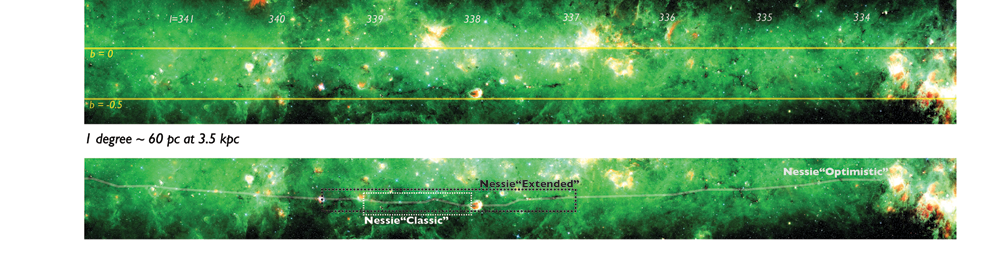
\includegraphics{figures/1nessie_findingchart/1nessie_findingchart.png}
\caption{image}
\end{figure}

\begin{figure}[htbp]
\centering
\includegraphics{figures/table1_mass_nessie/table1_mass_nessie.jpg}
\caption{image}
\end{figure}

\section{The Three-Dimensional Position of Nessie within the Milky Way}

{[}

3D{]}

\subsection{Looking ``Down" on the Galaxy}

{[}

lookingdown{]} Astronomers would love to travel far beyond the Milky
Way, so that we could observe its spiral pattern face-on, as we do for
other galaxies. But (the standard sad story goes) our Sun is so
entrenched in the Milky Way's plane that an ``overhead view" of the
Milky Way's structure is impossible. Or is it? What if the Sun were just
far enough above the Galactic Plane that we could use its height to give
ourselves a tiny bit of perspective on the Galactic Plane that would
spatially separate features--if they are very narrow--at different
distances to be at different projected latitudes? Turns out we
\emph{are} lucky in this way--the Sun \emph{is} apparently located a bit
above the Plane (see below), and we can use that vantage point to out
advantage.

To understand why most astronomers do not yet consider the possibility
or value of an overhead view, we need to consider the origin of our
current Galactic coordinate system, and our current understanding of the
Sun's and the Galactic Center's 3D positions. Writing in 1959 on behalf
of the International Astronomical Union's (IAU's) sub-commission 33b,
Blaauw et al. wrote:

\begin{quote}
The equatorial plane of the new co-ordinate system must of necessity
pass through the sun. It is a fortunate circumstance that, within the
observational uncertainty, both the sun and Sagittarius A lie in the
mean plane of the Galaxy as determined from hydrogen observations. If
the sun had not been so placed, points in the mean plane would not lie
on the galactic equator.

\end{quote}
In a further explanation of the IAU system in 1960, Blaauw et al.
explain that stellar observations did, at that time, indicate the Sun to
be at $z=22 \pm 2$ (22 pc above the plane), but the authors then
discount those observations as too dangerously affected by
hard-to-correct-for extinction in and near the Galactic Plane
\citep{BlaauwA.1960}. Instead, the 1959 IAU system relies on the 1950's
measurements of HI, which showed the Sun to be at $z=4\pm 12$ pc off the
Plane, consistent with the Sun being directly in the Plane ($z=0$).
Interestingly, since the 1950's, the Milky Way's HI layer has been shown
to have corrugations on the scale of 10's of pc \citep{Malhotra1995},
and there may be similar fluctuations in the mid-plane of the
${\rm H_2}$ \citep{Malhotra1994}, so it is still tricky to use gas
measurements to determine the Sun's height off the plane. xxBob/Tom D.
-- should we say more?xx

Astronomers today are still using the $(l^{II}, b^{II})$ Galactic
coordinate system defined by \citet{Blaauw1959}, but it is \emph{not}
still the case, within observational uncertainty, that the Sun is in the
mean plane of the Galaxy, and the true position of the Galactic Center
is no longer at $(l^{II}=0, b^{II}=0)$. Instead, a variety of lines of
evidence \citep{Chen2001b,Maiz-Apellaniz2001a,Juric2008a} show that the
Sun is approximately 25 pc above the stellar Galactic mid-plane, and
VLBA proper motion observations of masers show that the Galactic Center
is about 7 pc below where the $(l^{II}, b^{II})$ system would put it
\citep{Reid2004}. These offsets, as predicted by Blaauw et al., imply
that ``points in the mean plane {[}do{]} not lie on the galactic
equator."

Figure {[}fig:galcoords{]} shows a schematic (not-to-scale) diagram of
the effect of the Sun's and the Galactic Center's offsets from the
mid-plane defined by the IAU in 1959 (and still in use as
$(l^{II}, b^{II})$ today). The tilt of the ``True" Galactic Plane to the
presently IAU-defined Plane means that, within about 12 kpc of Sun
(Note: Twelve kpc is the approximate distance where the True and IAU
planes cross, on a line toward the Galactic Center. Along other
directions toward the Inner Galaxy, it will be further to the crossing
point, and toward the Outer Galaxy, the latitude of the Plane will
always be negative.) any feature that is truly ``in" the Galactic
mid-plane will appear on the Sky at negative $b^{II}$. Figure
{[}fig:coloredlines{]} shows an example of this effect, where the
rainbow-colored dashed line indicates the sky position of the ``True"
Galactic mid-plane at a Nessie-like distance of 3.1 kpc (assuming the
the Sun is 25 pc off the plane, a distance to SrgA* of 8.4 kpc, a
rotation speed for the Milky Way of 239 km~s$^{-1}$, and (U,V,W) motion
for the Sun of 11.1, 12.4, and 7.2 km~s$^{-1}$, respectively).

\begin{figure}[htbp]
\centering
\includegraphics{figures/2galactic_coords/2galactic_coords.jpg}
\caption{image}
\end{figure}

\subsection{Using Rotation Curves and Velocity Measurements to Place
Nessie in 3D}

Ever since velocity-resolved observations of stars and gas have been
possible, astronomers have been modeling the rotation pattern of the
Milky Way. Using a measured rotation curve for the Milky Way's gas,
e.g., \citep{McClureGriffiths2007}, one can translate observed LSR
velocities to a unique distance in the Outer Galaxy, and to one of two
possible (``Near" or ``Far") distances toward the Inner Galaxy. Figure
{[}fig:topview{]} shows iso-$v_{LSR}$ contours toward the Inner Galaxy,
around the longitude range of Nessie, superimposed on the data-driven
cartoon of our current understanding of the Milky Way's structure
(xxBenjamin will suggest how to reference this work by Hurt, Benjamin,
Dame, et al.xx). It is clear from Figure {[}fig:topview{]} why a
Near-Far distance ambiguity exists, and also that velocities associated
with the near-side of the Scutum-Centaurus Arm at Nessie's longitude
range should be near 40 km~s$^{-1}$.

Combining the modern measurements of the Sun's height above the plane
($z\sim 25$ pc), with the IAU galactic coordinate definitions as
described in Figure {[}fig:topview{]}, we can determine where the
mid-Plane of the Galaxy should appear in the $(l^{II}, b^{II})$ system
at any particular distance from the Sun. Figure {[}fig:coloredlines{]}
shows where the Scutum-Centaurus Arm would appear on the Sky (for a
distance to SrgA* of 8.4 kpc, a rotation speed for the Milky Way of 239
km~s$^{-1}$, and (U,V,W) motion for the Sun of 11.1, 12.4, and 7.2
km~s$^{-1}$, respectively). As its caption explains in detail, Figure
{[}fig:coloredlines{]}'s colored lines are associated with the near part
of the Scutum-Centaurus Arm (shown as short, yellow-greeen line segment
in Figure {[}fig:topview{]}). For reference, white lines in Figure
{[}fig:coloredlines{]} show the Sky position of the far part of the
Scutum-Centaurus arm in the same longitude range (shown as a white chalk
line in Figure {[}fig:topview{]}).

The dashed colored line in Figure {[}fig:coloredlines{]}, indicating the
predicted position of the Galactic Plane on the Sky at the distance to
the near side of the Scutum-Centaurus Arm, passes almost directly
through Nessie. Solid colored lines show 20 pc above and below the Plane
at the distance to the Scutum-Centaurus Arm, so Figure
{[}fig:coloredlines{]} makes it is very clear that Nessie lies within
just a few pc of the Plane, along its entire length. This is either an
extremely fortuitous coincidence, or an indication that Nessie is
tracing a significant feature that lies ``exactly" within the Galactic
Plane.

\emph{(CB NOTE): We've all mentioned this before, but I think it should
be in the paper: the location of Nessie within a few pc of the "mean" GP
is \textbf{both} a suggestion that Nessie lies exactly in the plane and
a coincidence. The plane is corrugated and wavy on ~10pc scales
according to the above text -- thus even if Nessie is exactly in the
local midplane, we are lucky that the local midplane lies so close to
the global midplane (i.e. the thing that the rainbow line traces) near
Nessie. I think it's important to note that we understand this fact,
lest a skeptic realize this as well and dismiss our argument}

\begin{figure}[htbp]
\centering
\includegraphics{figures/6drafttopview/6drafttopview.jpg}
\caption{image}
\end{figure}

\begin{figure}[htbp]
\centering
\includegraphics{figures/3draftnessie_vrad-2/3draftnessie_vrad-21.jpg}
\caption{image}
\end{figure}

\subsubsection{CO Velocities}

{[}

CO{]} CO observations trace gas with mean density around 100 cm$^{-3}$.
CO emission associated with the Scutum-Centaurus Arm of the Milky Way is
shown in Figure {[}fig:COarm{]}, which presents a plane-of-the-sky map
integrated over $-50 <v_{LSR}< -30$ km~s$^{-1}$. The velocity range is
centered on -40 km~s$^{-1}$, the average velocity of the
Scutum-Centaurus Arm in Nessie's longitude range (see Figures
{[}fig:topview{]} and {[}fig:coloredlines{]}). The white chalk line
superimposed on Figure {[}fig:COarm{]} is the same tracing of ``Nessie
Optimistic" shown in Figure {[}fig:FindingChart{]}. The black feature
labeled ``Nessie" refers to ``Nessie Classic."

The vertical (latitude) centroid of the CO emission attributed to the
Scutum-Centaurus Arm \citep{Dame2011} shown in Figure {[}fig:COarm{]}
appears to follow Nessie remarkably well, even out to the full $8^\circ$
(430 pc) extent of Nessie Optimistic. Table 1 estimates Nessie's typical
${\rm H_2}$ column density a $\gtrsim 10^{23}$ cm$^{-2}$ and its typical
volume density at $\gtrsim 10^5$ cm$^{-3}$. Thus, the plane-of-the-sky
coincidence of the line-of-sight-velocity-selected ``Scutum-Centaurus"
CO emission and the mid-IR extinction suggests that the Nessie IRDC may
be a kind of ``spine" or ``bone" of this section of the Scutum-Centaurus
Arm. But, the spatial resolution of the CO map is too low ($8'$), and
the 20 km~s$^{-1}$ velocity range associated with the Arm in CO is too
broad to decide based on this evidence alone whether Nessie is a
well-centered ``spine" or just a long skinny feature associated with,
but potentially significantly inclined to, the Scutum-Centaurus Arm.

CB NOTE: This claims in the last paragraph could be tested statistically
in a few different ways. The most obvious is to fit a moving-average
regression line through the CO map, and confirm that this line (+
uncertainties) overlaps Nessie. The second test is to check whether the
curvature in Nessie optimistic is present in the CO data (as the
paragraph seems to suggest). One could do this by fitting a straight
line through the CO data, and checking whether this is inconsistent with
the first regression line. I agree that these will probably be weak
tests given the intrinsic width of the CO data, but I would be in favor
of \emph{some} quantitative argument to back up the first sentence in
the previous paragraph. I could run these tests if someone points me to
the data used in the figure

\begin{figure}[htbp]
\centering
\includegraphics{figures/4draft_co_sky/4draft_co_sky.jpg}
\caption{image}
\end{figure}

\subsubsection{NH$_3$ Velocities}

{[}

ammonia{]} To estimate the 3D orientation of Nessie more precisely, we
need to employ a gas tracer whose emission is sparser than CO's in
position-position-velocity space. Many recent studies have shown that
IRDCs typically host over-dense blobs of gas (often called ``clumps" or
``cores") that provide the gaseous reservoirs for the formation for
massive stars. Thus, several studies have been undertaken to survey
IRDCs and their ilk for emission in molecular lines that trace
high-density ($\gg 10^3$ cm$^{-3}$), potentially star-forming, gas.

The H$_2$O Southern Galactic Plane (HOPS) Survey \citep{Purcell2012b}
has surveyed hundreds of sites of massive star formation visible from
the Southern Hemisphere for ${\rm NH}_3$ emission, which traces gas at
densities $n\gtrsim 10^4$ cm$^{-3}$. The HOPS targets were selected
based on H$_2$O maser emission, thermal molecular emission, and radio
recombination lines, so as to include nearly all known regions of
massive star formation within the surveyed area. These
``massive-star-forming region" selection criteria mean that the HOPS
database includes ${\rm NH}_3$ spectra for dozens of positions within
the longitude range covered by Nessie.

Figure {[}fig:HOPSoverlay{]} shows an overlay of HOPS sources
${\rm NH}_3$-determined LSR velocities on the Spitzer image of Nessie
used throughout this paper (see Figures {[}fig:FindingChart{]} and
{[}fig:coloredlines{]}). It is clear that the velocities of the HOPS
sources within Nessie Extended (xxshould we show more length of
Nessie?xx) agree remarkably well with what is predicted for the
Scutum-Centaurus Arm (color-coding of dashed line). The velocities of
sources at other latitudes within this longitude range do \emph{not}
agree, as they are not part of the Nessie feature, or, in most cases,
not even associated with the (near-side of the) Scutum-Centaurus Arm
(should we color-code the white lines, so we can show which of the
higher $b$ sources could be at the far part of the Arm? likely no,
because the sensitivity of HOPS should not really see many of those?xx).

For the innermost part of Nessie (Nessie Classic), Jackson et al. (2010)
had already noted a very narrow velocity range for dense gas associated
with the IRDC, based on HCN observations. What is new here is the
three-dimensional (latitude, longitude, and velocity) association of (an
even longer) Nessie's dense gas with predictions for where the centroid
of the Milky Way's Scutum-Centaurus Arm's ``middle" would lie. Figure
{[}fig:pvdiagram{]}, which offers a position-velocity diagram of CO and
${\rm NH}_3$ emission together, shows the association of the Nessie-HOPS
sources with the Scutum Centaurus Arm most clearly.

What is most remarkable about Figure {[}fig:pvdiagram{]} is that the
black line sloping through the figure is \emph{not} a fit to the black
dots representing the HOPS sources. Instead, that line indicated the
position-velocity trace of the Scutum-Centaurus Arm based on
\citep{Dame2011} data for the full Galaxy, not just this small longitude
range. Figure {[}fig:pvdiagram{]} implies that Nessie goes right down
the ``spine" of the Scutum-Centaurus Arm, as best we can measure its
position in CO position-velocity space.

\begin{figure}[htbp]
\centering
\includegraphics{figures/5draft_side_view/5draft_side_view.jpg}
\caption{image}
\end{figure}

\begin{figure}[htbp]
\centering
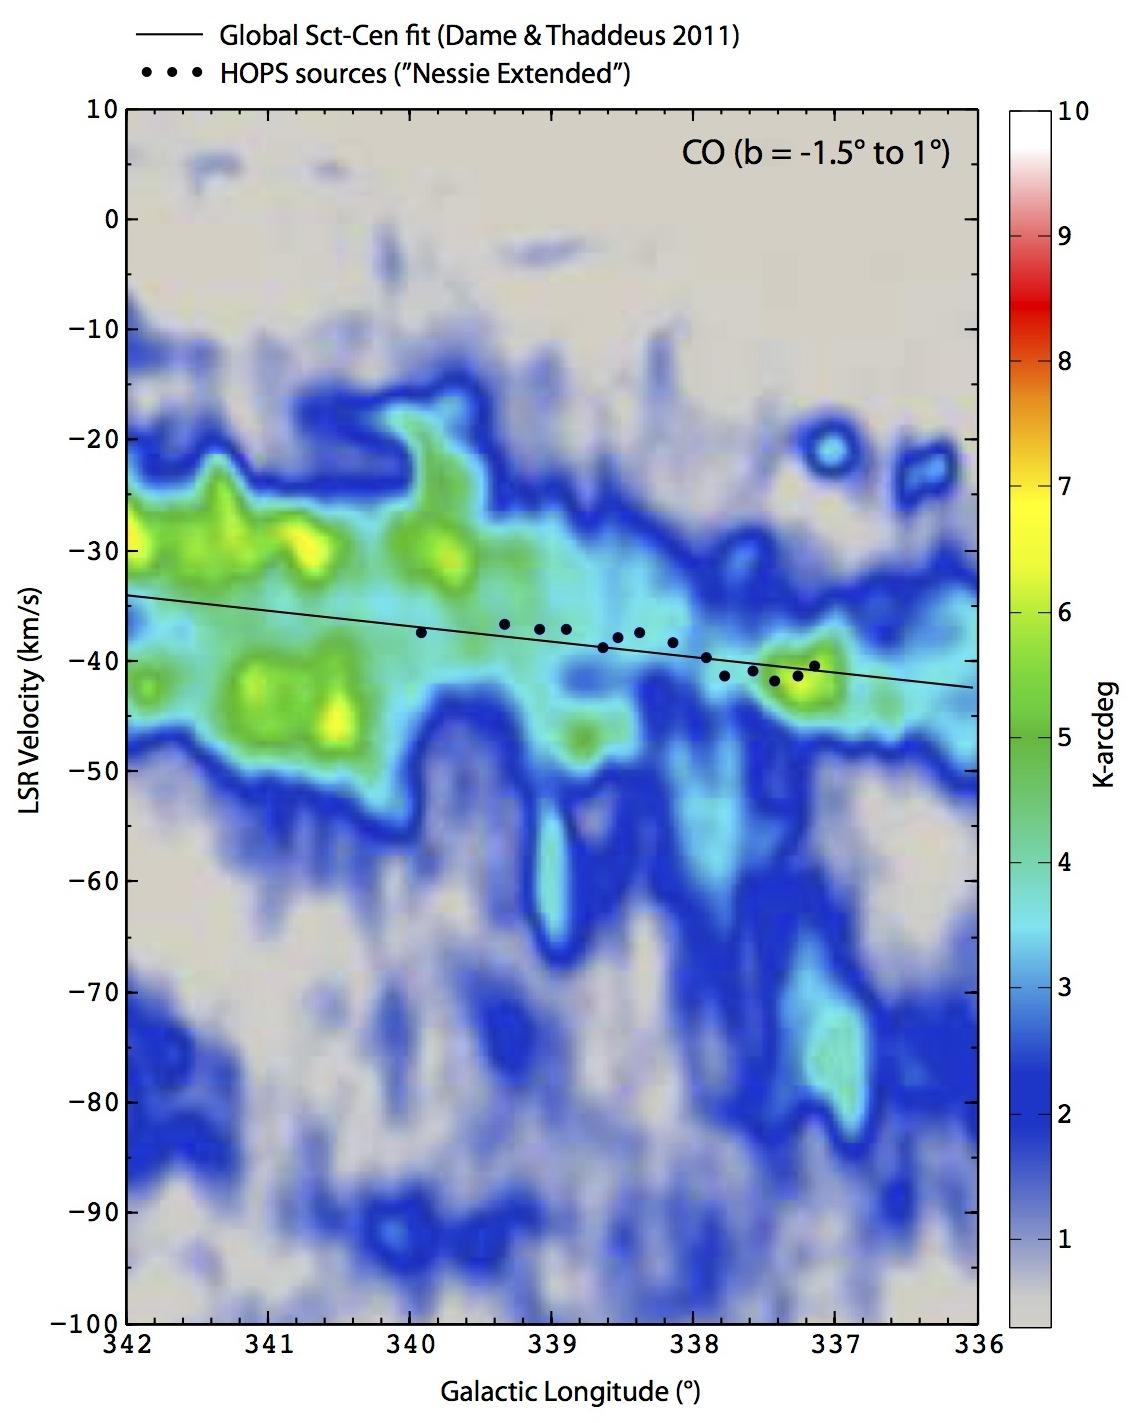
\includegraphics{figures/7draftNessie_CO_lv/7draftNessie_CO_lv.jpg}
\caption{image}
\end{figure}

\section{What is the Significance of Nessie-like structures within a
Spiral Galaxy?}

\subsection{A Bone of the Galaxy}

{[}

spine{]} All the evidence presented in this paper, taken together,
strongly suggests that Nessie forms a spine-like feature that runs down
the center of the Scutum-Centaurus Arm of the Milky Way. How did it get
there? Is it the crest of a classic spiral density wave \citep{Lin1964},
or does it have some other cause? Any feature this long and skinny that
is not controlled by Galactic-scale forces will be subject to a variety
of instabilities, and cannot last long. It would be great if we could
look to numerical simulations for answers, but today's simulations can,
alas, only give hints. Nessie is \emph{so} skinny, and \emph{so} much
denser than its surroundings that no extant numerical simulation has the
combination of spatial resolution and dynamic range in density needed to
produce a feature like it.

Figure {[}fig:simulation{]} offers a snapshot (available as a movie at
xxURLxx) of a numerical simulation (xxAndi: what is right Dobbs et al.
reference for simulation we are using, from
\url{http://empslocal.ex.ac.uk/people/staff/cld214/gmcs.html} xx) that
represents the state of the art at present. One can see density features
that are highly elongated, both within the spiral arms, and also between
the arms. Many of the features between the arms in Figure
{[}fig:simulation{]} are similar to the `spurs' and `feathers' that have
been simulated and observed by E. Ostriker and colleagues
\citep{Shetty2006, Vigne2008, Corder2008}. Figure {[}fig:IC342{]}
(discussed below) shows a recent WISE image of the galaxy IC342
\citep{Jarrett2013}, and it is clear from that image that some `spiral'
galaxies also exhibit inter-arm filaments that are even more pronounced
than the simulated spurs and feathers.

In the case of Nessie, the velocity information analyzed in §{[}CO{]}
and {[}ammonia{]} seems to very strongly favor Nessie's being oriented
exactly along (within, as the backbone of) an arm (Scutum-Centaurus)
over the idea that Nessie is a spur or interam filament.

{[}

Andi Burkert will further discuss the current limitations on simulation
resolution ... why can't we simulate Nessies yet? Andi will also say
more about the Dobbs' simulation's parameters and findings.{]}

The mass of Nessie under various assumptions is given in Table 1. If one
counts just the IRDC (infrared-opaque) part of Nessie, and so assumes a
mean density for the absorbing material of $10^5$ cm$^{-3}$, then Nessie
Classic is $4 \times 10^5$ M$_\odot$, Nessie Extended is $8 \times 10^5$
M$_\odot$ and Nessie Optimistic is $2 \times 10^6$ M$_\odot$. If one
assumes that the envelope traced by the HCN observations of Jackson et
al. (2010) for Nessie Classic continues along Nessie's length, then the
mass of a $n\sim 10^3$ cm$^{-3}$ cylindrical tube (see Table 1)
associated with Nessie would be $1.5 \times 10^6$ M$_\odot$ for Classic
and $4 \times 10^6$ M$_\odot$ for Optimistic. For the Optimistic case,
this mass amounts to 1/30,000th of the total baryonic mass (assuming
$\sim 10^{11}$ M$_\odot$ total) of the Milky Way, meaning that of order
1000's of additional Nessie-like features should be discoverable, if
they exist.

\begin{figure}[htbp]
\centering
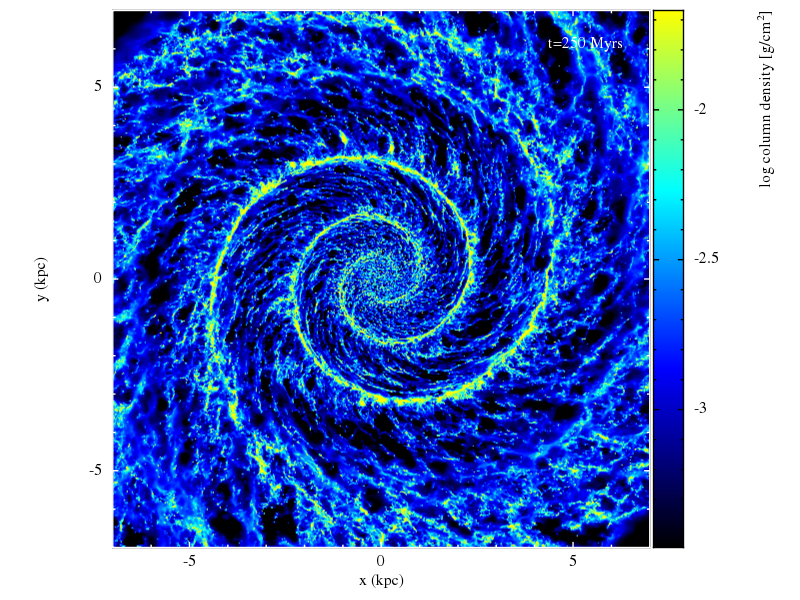
\includegraphics{figures/bones_dobbs/bones_dobbs.png}
\caption{image}
\end{figure}

\subsection{Can We Map the Full Skeleton of the Milky Way?}

{[}

future{]}

{[}

This section discusses the potential of combining the ``perspective"
offered by the Sun's height off the plane with very high resolution,
multi-band observations like what's given here to map out the full
skeleton of the Milky Way. Joao Alves will comment on extinction and
Herschel-like emission maps. Jens Kauffmann will also add comments.{]}

In an ideal Universe, we would be able to travel far enough outside of
the Milky Way to observe it from ``outside," the way that we see, for
example, Andromeda. The story for years has gone that generating an
observationally-based plan (overhead) view of the Milky Way is
impossible, because we are ``in" the Plane. It is if Earth-bound
astronomers have been living in the 2D world Edwin A. Abbott famously
called `Flatland \citep{Abbott2008} when it comes to thinking about how
to image the Milky Way's spiral structure. But, we can escape Flatland
by realizing that the tiny offset of the Sun above the Milky Way's
midplane can give us a tiny, but useful, bit of perspective on the 3D
structure of the Milky Way, and it can offer a (highly-foreshortened!)
overhead view. This perspective is only useful when looking at very
sharp, very narrow, features like Nessie, because puffier, more
standard, arm-defining features will overlap too much to be separated in
a very foreshortened view.

Carry out the following thought experiment. Draw a rough plan of a
spiral galaxy on a piece of paper. Position a vantage point a tiny
distance (a few hundredths of an inch) above that piece of paper, about
two-thirds of the way out from the center of the galaxy. Now give the
observer at that vantage point super-sharp eyesight and ask if the
observer can separate the spiral arm features you drew, as they observe
them. They can--if and only if the spiral you drew has very narrow
features defining its arms. If the observer were exactly \emph{in} the
piece of paper (living in Flatland), separating the arms would be
impossible, regardless of their width. We are, like your observer, are
at a tiny, tiny, elevation off of a spiral galaxy, and our visiion is
good enough to separate very skinny arm-like features.

So, how might we use out vantage point above the Plane to map out more
of the Milky Way's skeleton? It turns out that Nessie is located in a
place where seeing a very long IRDC projected parallel to the Galactic
Plane should be just about the easiest, so it is not surprising that we
found it first. Look again at Figure {[}fig:topview{]}, and consider
Nessie's placement there (the yellow-green line). According to the
current (data-based cartoon) view of the Milky Way shown in Figure
{[}fig:topview{]}, Nessie is in the closest major spiral arm
(Scutum-Centaurus) to us, along a direction toward, but not exactly
toward, the (confusing) Galactic Center. Nessie's placement there means
that it will have a bright background illumination as seen from futhrer
out in the Galaxy (e.g. from the Sun), and that it will have a long
extent on the Sky as compared with more distant or less
perpendicular-to-our-line-of-sight objects.

To find more `Nessies,' if such narrow features are in fact typical in
spiral arms, we need to be clever about where and how we look. Our
current understanding of the Milky Way's spatial and velocity structure
will allow us to draw more velocity-encoded lines like the ones shown in
Figure {[}fig:coloredlines{]} on the Sky, mapping out the whole Galaxy
as seen from the Sun's vantage point. Once this drawing is done, we
should design algorithms to look for dust clouds elongated (roughly)
along those lines, and then we should examine the velocity structure of
the elongated features, as we do in §{[}3D{]}, above. Of course, we need
to be flexible in which features we accept as possible other ``bones,"
remembering that the model we will use to draw the expected features on
the Sky is the same one we seek to refine! It is likely that a Bayesian
approach, using the extant Milky Way model as a prior, will succeeed in
this way.

As extinction {[}xxJoaoxx{]} and dust emission {[}xx Tom R.,
Jensxx{]}data cover more and more of the sky at ever-improving
resolution and sensitivity, we should be able to map more and more of
the Milky Way's skeleton.

Recent (e.g. Spitzer, Herschel) mid- and far-infrared imagery already
suggests that: 1) not all galaxies once thought to be dominated by a
spiral pattern really are; and 2) not all IRDCs are likely to be part of
the Milky Way's skeleton.

As mentioned above, images like Figure {[}fig:IC342{]} clearly show that
spiral galaxies can be very web-like, with long, straight filaments
interconnecting spiral arms. {[}xxJens--add comments about dark lanes in
other galaxies near here.xx{]} Thus, some of the features seen as long,
skinny, IRDCs in the Milky Way could very well \emph{not} be part of
spiral arms, even if they are part of a Galaxy-wide structural pattern.
This possibility will clearly complicate the modeling discussed above,
but that just makes it more interesting! New data from ever-deeper and
ever-sharper extragalactic observations will likely reveal even more
complex galaxy strucutres. Combining ALMA thermal dust emission and
molecular line observations of slightly-inclined galaxies will allow us
to combine structural image with velocity information facilitating
ever-improving model comparison.

Over the past 15 years, since their discovery, there have been many
efforts to catalog and characterize IRDCs, and it is clear that not all
IRDCs are, or should be, part of Nessie-like bones.

The catalog compiled by \citet{Peretto2009a} lists 11,000 IRDCs, but
none of the features cataloged will be Nessie-like on its own. The
structure-finding algorithm used in the Peretto \& Fuller work is biased
toward finding core-like roundish peaks, so a cloud like Nessie forms a
connect-the-dots pattern (xxcould show figure like the one in WWT Tour
with all the dots?xx) in the Peretto \& Fuller catalog. In fact, Nessie
is comprised of xxroughly 35xx Peretto \& Fuller sources. So, while the
Peretto \& Fuller catalog is tremendously useful to the study of the
properties of massive star forming cores, it will only become useful for
finding ``bones" when someone applies a clever dot-connecting algorithm
to it, and its ilk.

Some very large, and/or very extended, IRDCs, such as the so-called
``Massive Molecular Filament" studied by \citet{Battersby} xxdetails
from Jens or AGxx, are not located along the plane-of-the-sky projected
spiral arms. These clouds, which are probably just massive star-forming
regions near but not exactly in the Galactic plane, do not appear as
straight or highly-elongated as Nessie, and they may offer a hint at
what threshold to set in looking for elongated features as we search for
more bones. Futher, once numerical galaxy-simulation modeling resolution
catches up to observational resolution, models should be able to say
whether they other, non-bone-like, massive IRDCs had their origins long
ago in bones, or form in some other way.

xx(and any other relevant new work?)xx

\begin{figure}[htbp]
\centering
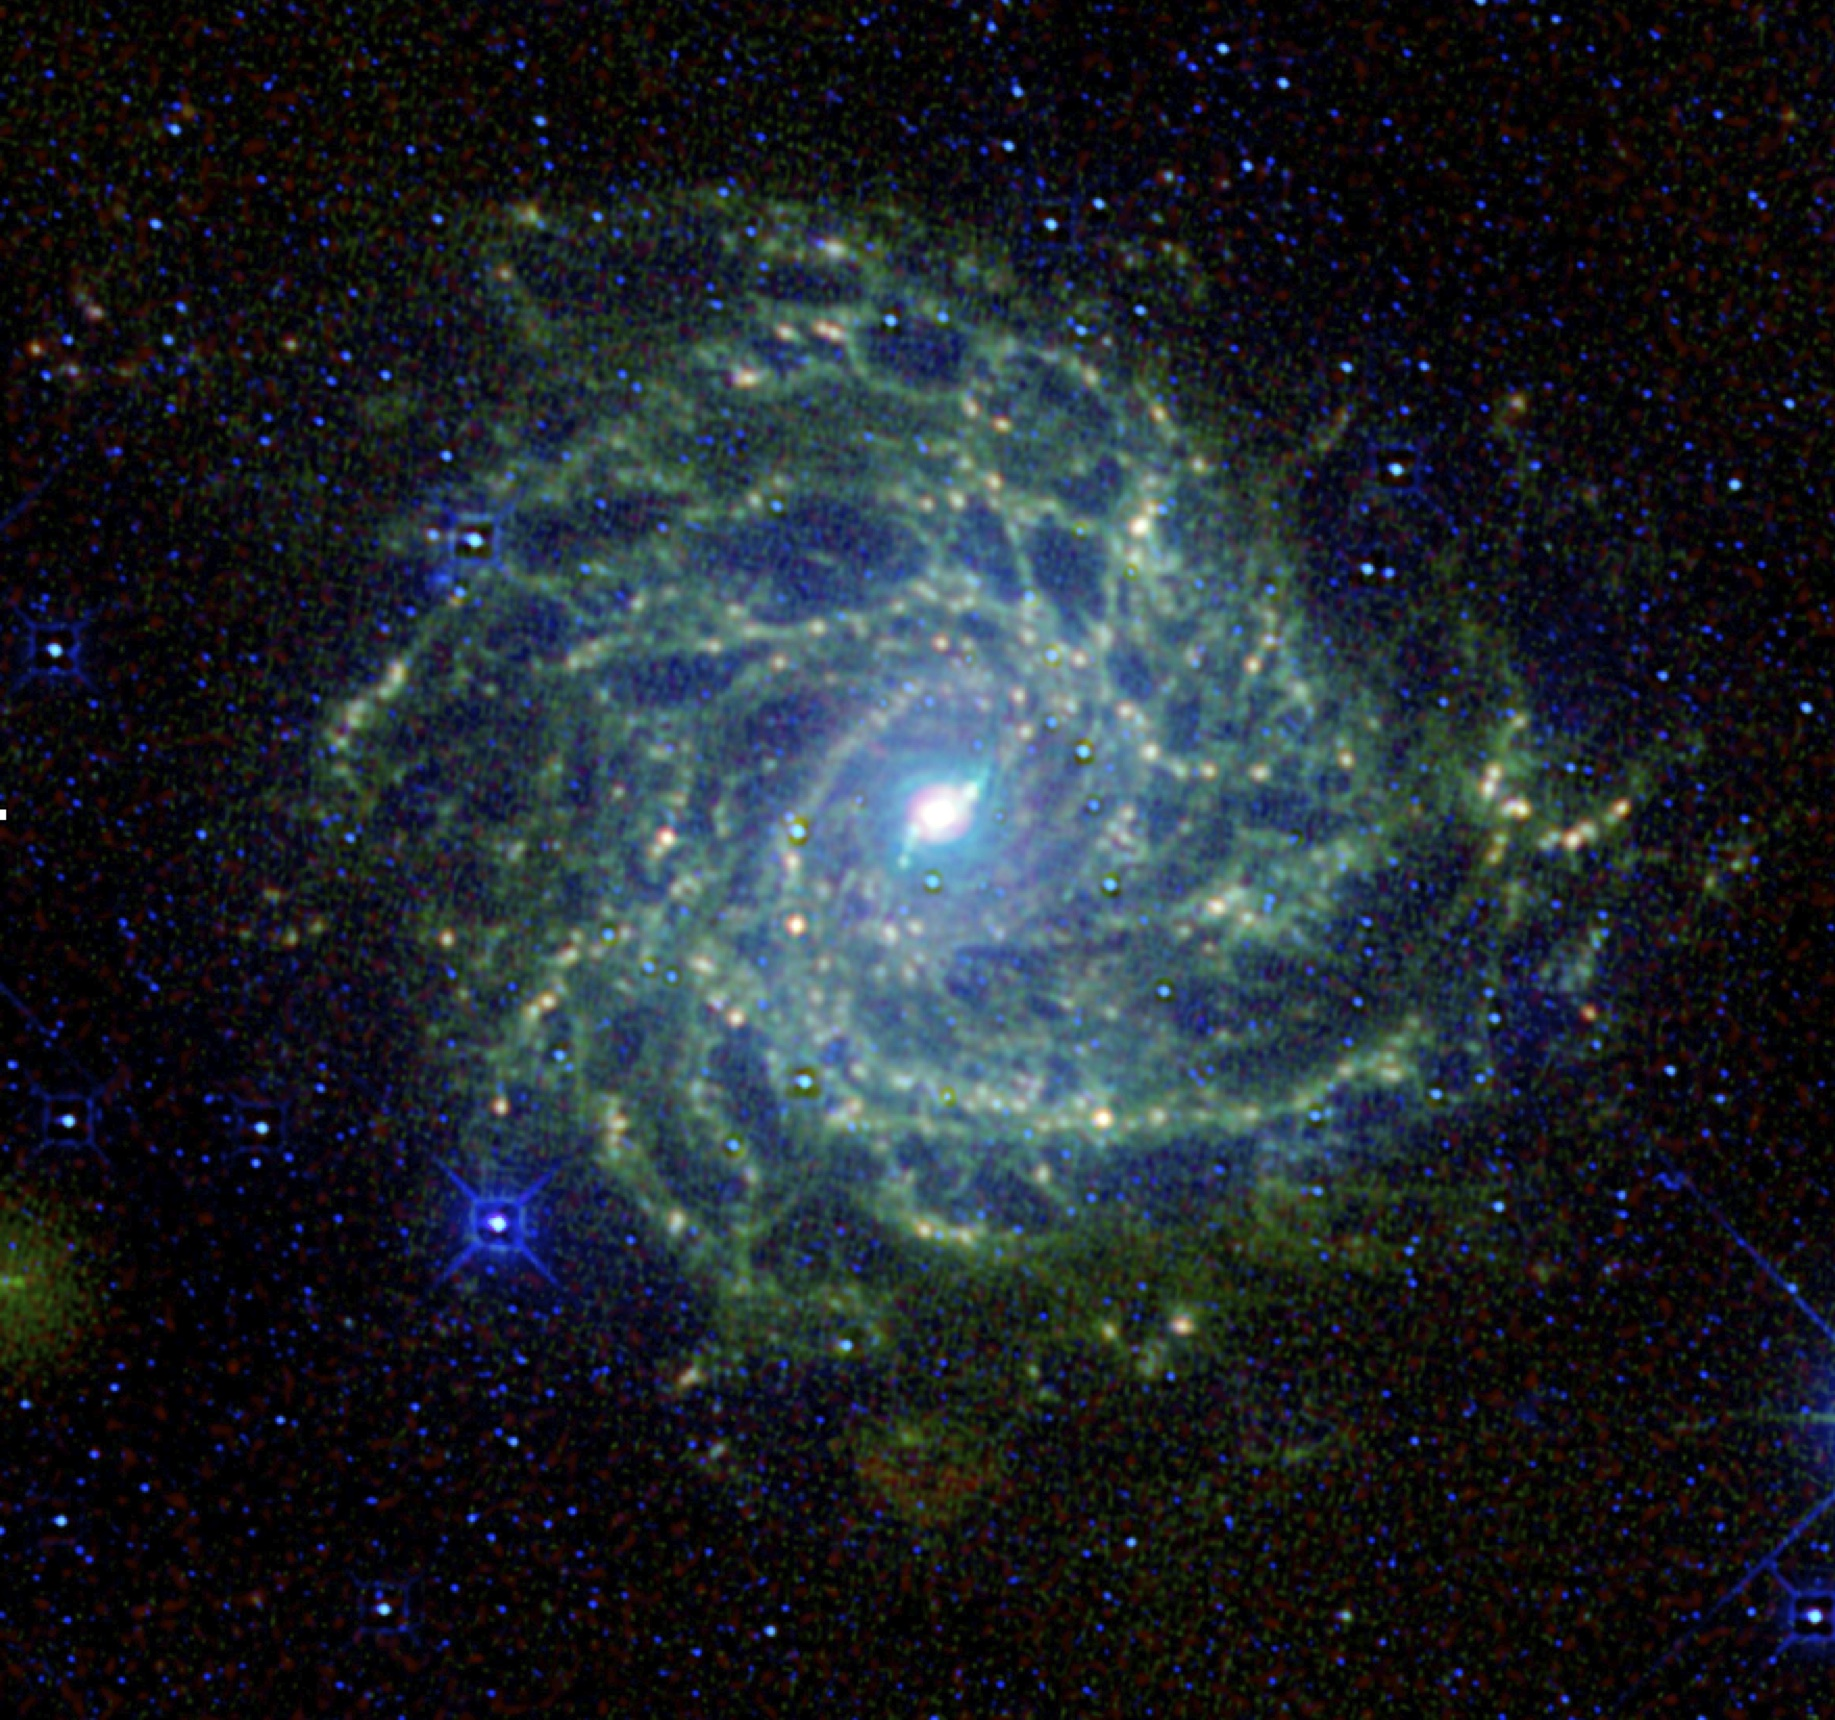
\includegraphics{figures/9ic342_jarrett_lowres/9ic342_jarrett_lowres.jpg}
\caption{image}
\end{figure}

\section{Conclusion}

xxDo we need a separate concluding section?xx

\subsection{Contributions}

This paper was a truly a group effort, and the author list includes only
some of the many people who have contributed to it. The entire project
was inspired by a question: ``Is Nessie parallel to the Galactic
Plane?," asked by Andi Burkert at the 2012 Early Phases of Star
Formation (EPoS) meeting at the Max Planck Society's Ringberg Castle in
Bavaria. Three EPoS attendees beyond the author list contributed
significant ideas and data to this work, most notably Steven Longmore,
Eli Bressert, and Henrik Beuther. We are grateful to Cormac Purcell for
giving us advance online access to the HOPS data, and to Mark Reid for
generously sharing his expertise on Galactic structure. The text here
was largely written by Alyssa Goodman; the theoretical ideas come
primarily from Andi Burkert; and much of the geometrical analysis was
carried out by Christopher Beaumont, Bob Benjamin, and Tom Robitaille.
Tom Dame and Bob Benjamin provided expertise on Galactic structure, and
they created several of the figures shown here. Jens Kauffmann provided
expertise on IRDCs, and also was first to point out the potential
relevance of the Sun's non-zero height above the Galactic Plane. Joao
Alves provided expertise on the potential for using extinction maps to
find more Nessie-like features, and Michelle Borkin was instrumental in
early visualization work that led to our present proposals for using the
Sun's ``high" vantage point to map out the Milky Way. Jim Jackson
contributed critical expertise on the Nessie IRDC, based both on the
2010 study he led and on unpublished work since. xxacknowledge NSF and
NASAxx xxAdd here or in appropriate funding blurb spot: ``M. Borkin was
supported by the Department of Defense through the National Defense
Science \& Engineering Graduate Fellowship (NDSEG) Program.'' xx

\subsection{Facilities}

(xxcheck current ApJ format, namesxx) MOPRA, CfA Mini, Spitzer Space
Telescope.

\end{document}

